\graphicspath{{CPE/Star2/image/}}
\subsection{UVa679 - Dropping Balls}
A number of $K$ balls are dropped one by from the root of a fully binary tree structure FBT. Each time the ball begin dropped first visits a non-terminal node. It then keeps moving down, either follows the path of the left subtree, or follows the path of the right subtree, until it stops at one of the leaf nodes of FBT. To determine a ball's moving direction a flag is set up in every non-terminal node with two values, either \textbf{false} or \textbf{true}. Initially, all of the flags are \textbf{false}. When visiting a non-terminal node if the flag's current value at this node is \textbf{false}, then the ball will first switch this flag's value, i.e., from the \textbf{false} or \textbf{true}, and then follow the left subtree of this node to keep moving down. Otherwise, it will also swith this flag's value, i.e., from the \textbf{true} to the \textbf{false}, but will follow the right subtree of this node to keep moving down. Futhermore, all nodes of FBT are sequentially numbered, starting at 1 with nodes on depth 1, and then those on depth 2, and so on. Nodes on any depth are numbered from left to right.

For example, Fig. 1 represents a fully binary tree of maximun depth 4 with the node numbers 1, 2, 3, ..., 15. Since all of the flags are initially set to be false, the first ball being dropped will switch flag's values at node 1, node 2, and node 4 before it finally stops at position 8. The second ball being dropped will switch flag's values at node 1, node 3, and node 6, and stop at position 12. Obviously, the third ball being deopped will switch flag's values at node 1, node 2, and node 5 before it stops at position 10.

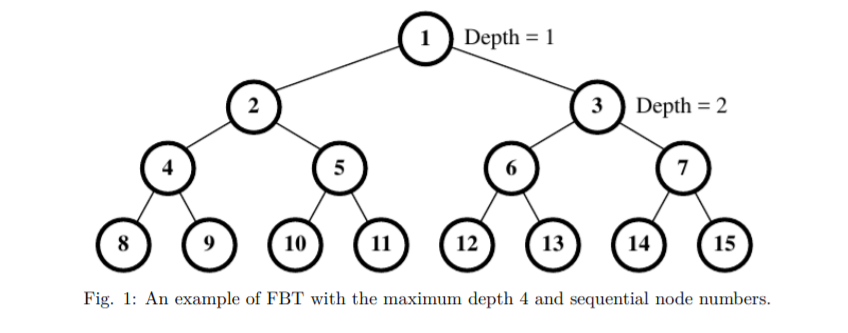
\includegraphics[width=\textwidth]{UVa679}

Now consider a number of test cases where tow values will be given for each test. The first value is $D$, the maximum depth of FBT, and the second one is $I$, the $I$-th ball being deopped. You may assume the value of $I$ will not exceed the total number of leaf nodes for the given FBT.

Please write a program to determine the stop position $P$ for each test case.

For each test cases the range of two parameters $D$ and $I$ is as below:
\[ 2 \leq  D \leq 20 , \ and \ 1 \leq I \leq 524288  \]

\begin{flushleft}
{\color{red} \textbf{Input}}
\end{flushleft}
\begin{flushleft}
Contains $l+2$ lines.\\
Line $1$ \quad $l$ \quad the number of test cases\\
Line $2$ \quad $D_1 I_1$ \quad test case \#1, tow decimal numbers that are separated by one blank\\
...\\
Line $k$ \quad $D_k I_k$ \quad test case \#k\\
Line $l$+1 \quad $D_l I_l$ \quad test case \#l\\
Line $l$+2 \quad $-1$ \quad a constant '-1' representing the end of the input file\\
\end{flushleft}

\begin{flushleft}
{\color{red} \textbf{Output}}
\end{flushleft}
\begin{flushleft}
Contain $l$ lines.\\
Line $1$ \quad the stop position $P$ for the test case $\#1$\\
...\\
Line $k$ \quad the stop position $P$ for the test case $\#k$\\
...\\
Line $l$ \quad the stop position $P$ for the test case $\#l$\\
\end{flushleft}

\begin{flushleft}
{\color{red} \textbf{Sample Input}}
\end{flushleft}
\begin{flushleft}
5\\
4 2\\
3 4\\
10 1\\
2 2\\
8 128\\
-1\\
\end{flushleft}

\begin{flushleft}
{\color{red} \textbf{Sample Output}}
\end{flushleft}
\begin{flushleft}
12\\
7\\
512\\
3\\
255\\
\end{flushleft}

\newpage